\chapter{Draft}

\section{RQ1. Com que frequência \textit{breaking changes} surgem nos pacotes clientes?}
\label{sec:rq1}

\subsection{Motivação}
\label{mot:rq1}

No ecossistema do \gls{NPM}, uma simples \textit{release} que contenha um erro pode afetar uma quantidade imensa de pacotes, uma vez que este repositório contém a maior rede de dependências entre pacotes \cite{teorical_reference:npm_2}. Para evitar que \textit{breaking changes} se manifestem nos pacotes clientes, os provedores introduzem as \textit{breaking changes} em \textit{releases major}, seguindo o padrão do Versionamento Semântico, e os cliente podem utilizar \textit{strings semver} para aceitar apenas as versões \textit{minor} e \textit{patch} dos provedores, o que é o padrão do \gls{NPM}. Entretanto, nem sempre o provedor é capaz de distinguir se suas alterações são \textit{breaking} ou \textit{non-breaking changes} \cite{noregrets2018}, ou, muitas vezes, as \textit{breaking changes} são introduzidas sem que o provedores percebam. Portanto, quando as \textit{breaking changes} são introduzidas em \textit{releases minor} ou \textit{patch}, elas podem causar comportamentos inesperados no cliente. Nesta RQ, queremos quantificar as manifestações das \textit{breaking changes} nos pacotes clientes. Assim, entender a frequência que os provedores publicam \textit{breaking changes} que afetam os clientes pode ajudar os clientes a fazer decisões melhores sobre como e quando atualizar a versão do seu provedor.

\subsection{Método}
\label{apr:rq1}

%\Gls{NPM}.
Um \textit{stack trace} é utilizado pelo \gls{NPM} para apresentar informações sobre um determinado erro. Quando os comandos \textit{npm install} e \textit{npm test} resultam em erro, o \Gls{NPM} mostra o erro e todas as chamadas de função, incluindo as invocações para os provedores. A Figura \ref{fig:trace} mostra um exemplo genérico de um \textit{stack trace} exibido pelo \Gls{NPM}. Nesta Figura, no topo do \textit{stack trace}, contém o tipo do erro que interrompeu a execução e a sua mensagem. Nas linhas abaixo, há todas as funções e arquivos que foram executados até a manifestação do erro. Com todos estes dados, o \textit{stack trace} auxilia no rastreamento de cada erro, uma vez que ele será utilizado para detectar as \textit{breaking changes}, pois através do \textit{stack trace} é possível identificar exatamente onde o erro se manifestou: no ciente ou no provedor.

\begin{figure}
    \centering
    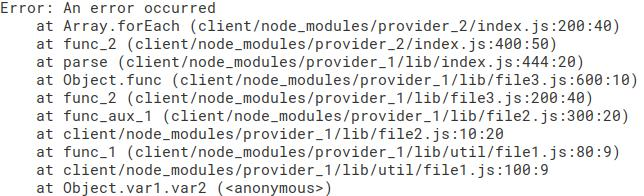
\includegraphics[scale=0.7]{figuras/stack_trace.jpeg}
    \caption{Generic stack-trace}
    \label{fig:trace}
\end{figure}{}

O \textit{stack trace} é a base da analise de um erro. A primeira etapa da análise de um erro é diferenciar entre um erro que foi causado pelo próprio pacote cliente, no qual não houve influência de nenhum provedor, e um erro que foi causado por algum dos provedores, sendo assim uma \textit{breaking change}.

Quando não há registro de execução dos provedores no \textit{stack trace}, provavelmente o erro não foi causado por uma \textit{breaking change}. Assim, o erro pode estar apenas no código do cliente. Para confirmar isto, foi procurado no \textit{GitHub} do cliente pelos próximos \textit{commits} após a data da \textit{release} no qual o cliente tenta consertar algum erro. Se foi encontrado algum \textit{commit} com correções, foi feita estas alterações no código do cliente para verificar se as modificações encontradas no \textit{GitHub} realmente refletem a correção do erro. Assim, se as alterações apenas no código do cliente refletir na correção do erro, sem que haja influência dos provedores, então o erro não se trata de uma \textit{breaking change}.

%evidência
Quando há registro da execução dos provedores no \textit{stack trace}, o erro provavelmente se trata de uma \textit{breaking change}. Entretanto, as chamadas para \textit{frameworks} de teste, como o \textit{Mocha\footnote{https://www.npmjs.com/package/mocha}, Jasmine\footnote{https://www.npmjs.com/package/jasmine}} entre outros, ou automatizadores de tarefas, como o \textit{Grunt\footnote{https://www.npmjs.com/package/grunt}} por exemplo, não evidenciam, inicialmente, a presença de \textit{breaking changes} uma vez que eles apenas iniciam a execução do pacote. Porém, não foi descartados a hipótese de apresentarem \textit{breaking changes}.

O melhor local para se confirmar a existência da \textit{breaking change} é no \textit{GitHub} e várias técnicas foram utilizadas para recuperar as informações necessárias. A seguir, encontra-se os métodos utilizados para detectar as \textit{breaking changes}:

\begin{itemize}
    \item Arquivos de alterações: os arquivos de registros de alterações, comumente nomeados por \textit{CHANGELOG.md} ou \textit{HISTORY.md}, contêm as descrições das principais alterações em cada \textit{releases} do projeto. Através da versão do provedor que foi descarregada do \gls{NPM}, é possível verificar nos arquivos de alterações quais foram as modificações introduzidas pelos provedores e se alguma destas alterações diz respeito ao erro encontrado no cliente. Uma das informações mais relevantes nestes arquivos são as descrições de \textit{breaking changes}. Por exemplo, a versão \textit{5.0.0} do pacote \textit{Mocha} contém uma \textit{breaking change} que foi documentada no \textit{CHANGELOG.md}\footnote{https://github.com/mochajs/mocha/blob/master/CHANGELOG.md\#500--2018-01-17} de acordo com a Figura \ref{fig:bc_documentation} (a). Outro tipo de documentação equivalente são as \textit{releases-notes}, como pode ser visualizado na Figura \ref{fig:bc_documentation} (b) como o pacote \textit{wpxml2md} documentou \textit{breaking changes} nas \textit{releases-notes}\footnote{https://github.com/akabekobeko/npm-wpxml2md/releases/tag/v2.0.0}. Entretanto, apenas 46\% dos repositórios utilizados nesta pesquisa contêm algum dos dois registros.

    \item \textit{Issues/Pull-requests}: uma vez que uma \textit{breaking change} se manifesta em algum cliente, ele pode -- e deve -- registrar este erro através de uma \textit{issue} no repositório do provedor. O proveito de buscar informações nas \textit{issues} é que essas contêm comentários dos provedores e da comunidade, assim, há muitas informações sobre um determinado erro, além de várias outras \textit{issues} lincadas, ampliando a busca por informações. Da mesma maneira os \textit{pull-requests} foram utilizados para buscar informações sobre as \textit{breaking changes}.

    \item Versões prévias dos provedores: um ponto muito importante é a instalação de versões prévias dos provedores. Uma vez que foi identificado qual provedor está causando a \textit{breaking change}, a instalação de outras versões ajudam a descobrir a partir de qual \textit{release} do provedor a \textit{breaking change} foi introduzida, ou a partir de qual \textit{release} ela foi consertada. Com isso, a \textit{breaking change} fica mais fácil de ser identificada.

    \item Ferramentas \textit{diff}: o uso da ferramenta que realizam o  \textit{diff} entre duas \textit{releases} de um pacote foi muito importante. Foi utilizado a ferramenta \textit{npm-diff}\footnote{https://github.com/danielventurini/npm-diff}. Com isso, foi possível verificar o que foi adicionado e removido do código do provedor -- até mesmo do cliente -- em um determinado intervalo de versões.

    \item Sistemas integrados ao \textit{GitHub}: alguns sistemas integrados ao \textit{GitHub} auxiliam na investigação. Esses sistemas são o \textit{Travis\footnote{https://travis-ci.org}, Codeship\footnote{https://codeship.com}} entre outros que armazenam os resultados da execução do pacote para cada \textit{commit}. Eles são usados da seguinte maneira: se nesses sistemas integrados, a execução do pacote no \textit{commit} da \textit{release} do cliente foi realizado sucesso e, ao executá-los nesta pesquisa, resultou em erro, significa que há uma \textit{breaking change}, uma vez que o código do cliente está na mesma \textit{working tree} do \textit{commit}. Mas, se a execução do pacote cliente no momento do \textit{commit} resultou em erro, provavelmente os próximos \textit{commits} contêm alguma informação sobre o erro e sua correção, uma vez que estes sistemas integrados avisam os desenvolvedores sobre o erro na execução.
\end{itemize}

\begin{figure}
    \centering
    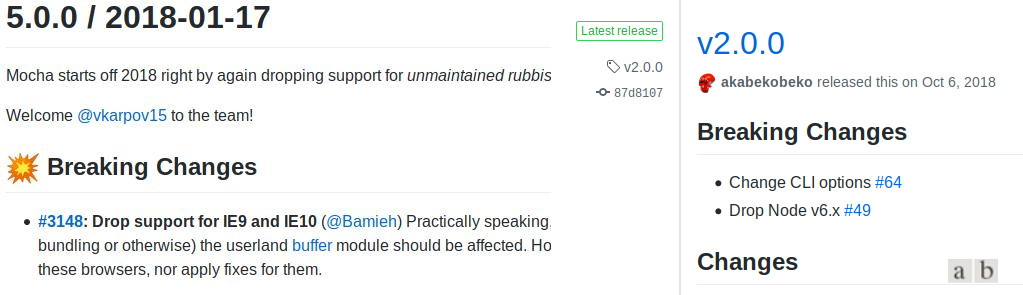
\includegraphics[scale=0.45]{figuras/bc_documentation.jpeg}
    \caption{Documentação de uma \textit{breaking change} no \textit{CHANGELOG} e nas \textit{release-notes}}
    \label{fig:bc_documentation}
\end{figure}{}

%Vale ressaltar que alguns sistemas integrados ao \textit{GitHub} auxiliaram na investigação. Esses sistemas são o \textit{Travis, Jenkins, Codeship, CicleCI} etc. Eles colaboraram ...

Um detalhe importante se refere aos pactes que utilizavam algum tipo de sistemas terceiros como o \textit{MySql\footnote{https://www.mysql.com}, Redis\footnote{https://redis.io}} entre outros. Então, quando foi gerado um erro pela falta de um destes sistemas, fez-se a habilitação e o pacote foi re-executado.

A Figura \ref{fig:step_analyze} exemplifica as técnicas utilizadas para responder esta questão de pesquisa.

\begin{figure}
    \centering
    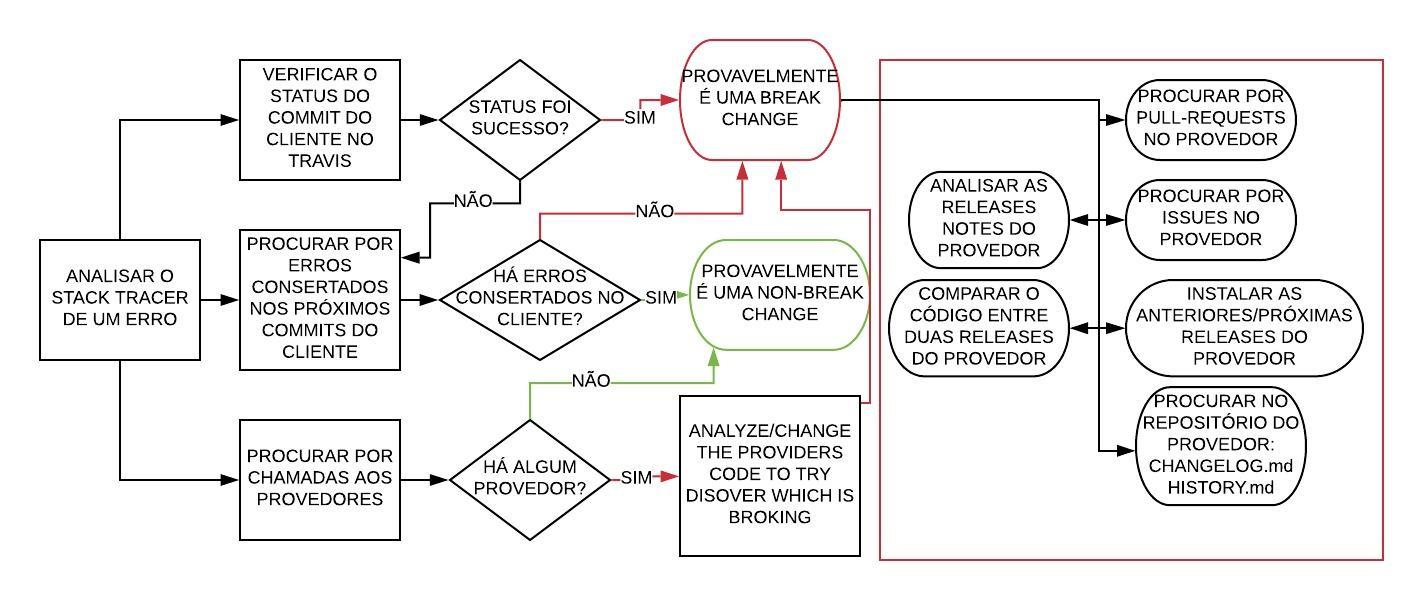
\includegraphics[scale=0.73]{figuras/step_analyze_pt.jpeg}
    \caption{Passos para analisar um erro}
    \label{fig:step_analyze}
\end{figure}

Então, para todas as \textit{releases} analisadas manualmente, foi salvo as seguintes informações para que fosse possível quantificar as \textit{breaking changes} e responder as demais questões de pesquisas:

\begin{enumerate}
    \item Em que local o erro foi documentado: \textit{issue, changelog, pull-request} etc;
    \item Quem consertou o erro: cliente ou providor;
    \item Em qual nível do \textit{SEMVER} o erro foi reparado;
    \item Quanto tempo o erro levou até ser corrigido; e
    \item Por quantas \textit{releases} o erro persistiu.
\end{enumerate}{}

\subsection{Resultados}
\label{fin:rq1}

\subsubsection{De todos os pacotes, 11\% foram impactados por \textit{breaking changes}}

\subsubsection{De todos os pacotes afetados, 13\% apresentaram mais de uma \textit{breaking change}}

%---------------------------------------------------%
\section{RQ2. Como os pacotes provedores introduzem \textit{breaking change} em uma \textit{release}?}
\label{sec:rq2}

\subsection{Motivação}
\label{mot:rq2}
Os tipos de \textit{breaking changes} são variados e podem se manifestar desde uma remoção/renomeação de uma \gls{API} até uma alteração do tipo de objeto retorno ao cliente. Em linguagens tipadas, a alteração da lista de parâmetros de uma função, por exemplo, é facilmente detectável e logo impossibilita a execução do código. Já em linguagens dinâmicas como o \textit{Javascript}, esta \textit{break change} nem se manifesta -- o \textit{Node.js} executa o código \textit{Javascript} sem se preocupar com lista de parâmetros. Desta maneira, algumas \textit{breaking changes} em \textit{Javascript} são diferentes das \textit{breaking changes} nas demais linguagens de programação. Assim, grande parte das \textit{breaking changes} em \textit{Javascript} são detectadas apenas em tempo de execução \cite{noregrets2018}, mas para o cliente, ter seu código encerrado em tempo de execução pode ser muito custoso. Por isso, dimensionar e categorizar as \textit{breaking changes} ajudará os desenvolvedores a atentar-se para as \textit{breaking changes} mais comuns e tentar evitá-las, assim produzindo códigos menos favoráveis às \textit{breaking changes}.

\subsection{Método}
\label{apr:rq2}

O objetivo da análise manual é descobrir o motivo que originou uma \textit{breaking change}, ou seja, qual foi a alteração que o provedor realizou que causou a \textit{breaking change} para que seja possível agrupa-las por suas similaridades. A análise manual é essencial, pois o \textit{stack trace} sempre apresenta o erro de uma maneira genérica. Então, as vezes, a mensagem de erro pode induzir a interpretação errônea do real motivo que originou a falha.

Cada caso de \textit{breaking change} será analisado e motivo que levou a sua manifestação será anotado para ser comparado com os demais. Após descobrir que um erro diz respeito à alteração de \gls{API}, por exemplo, uma categoria chamada \textit{Função Renomeada} será criada e as demais \textit{breaking changes} que possuem características comuns a esta também serão categorizadas como \textit{Função Renomeada}. Assim será possível quantificar cada uma das categorias. E mesmo processo será realizado para as demais \textit{breaking changes}, sempre visando criar categorias da maneira mais genérica que agrupe os erros semelhantes.

\subsection{Findings}
\label{fin:rq2}

%---------------------------------------------------%
\section{RQ3. Como os pacotes clientes se recuperam das breaking change?}
\label{sec:rq3}

\subsection{Motivação}
\label{mot:rq3}
Uma vez que uma \textit{breaking change} é introduzida, o cliente deve se recuperar dessa. Isso se faz necessário pois, no ecossistema \gls{NPM}, no qual centenas de milhares de pacotes estão conectados, uma simples \textit{release} com erro pode ocasionar na quebra de muitos clientes. No entanto, como os provedores evoluem independentemente dos clientes, erros e vulnerabilidades são difíceis de rastrear e corrigir nos clientes. Mesmo quando as vulnerabilidades podem ser corrigidas com a atualização para uma versão mais recente do provedor, pode haver incompatibilidades de \textit{API} -- entre outras incompatibilidades -- com os clientes que deve ser resolvido manualmente \cite{Foo:2018:ESC:3236024.3275535}. Desta maneira, entender como o cliente reage às \textit{breaking changes} ajudará os próprios clientes e os provedores a conhecerem as alternativas frente a uma \textit{breaking change} para que os clientes possam se recuperar da maneira mais eficiente.

\subsection{Método}
\label{apr:rq3}
Uma vez que os clientes se recuperaram de um erro, há duas maneiras para se obter informações sobre esta recuperação. A primeira maneira é quando o provedor corrige seu código e o cliente apenas atualiza sua \textit{string} de versionamento no \textit{package.json}, se precisar. Para o provedor consertar o erro, deve haver uma \textit{issue} no seu repositório. A segunda maneira é quando o próprio cliente conserta o código. Neste caso, o cliente pode corrigir o código do provedor e realizar um \textit{pull-request}. Também, o cliente pode alterar apenas o seu código para que execute normalmente com a \textit{release} errônea do provedor. Há casos também no qual nem o cliente nem o provedor faz nada para consertar o erro.

Todas as informações sobre esta questão de pesquisa foram recuperadas do \textit{GitHub}. As informações foram encontradas em \textit{CHANGELOGs, release-notes, issues} e \textit{pull-requests}. Os \textit{CHANGELOGs} contêm informações sobre os erros consertados. A partir das \textit{issues} é possível entender com os comentários dos clientes quais foram as ações que eles realizaram para se recuperar de uma determinada \textit{breaking change}. Pois, assim como o código de um pacote fica emaranhado com o código no restante do ecossistema ao qual ele pertence, o mesmo acontece com as \textit{issues}. Uma manifestação disso é que muitas \textit{issues} abertas em um projeto são vinculadas a \textit{issues} relacionadas, em projetos iguais ou diferentes, pois os desenvolvedores estão rastreando as causas de um problema \cite{Zhang:2018:WIL:3242887.3242891}. De maneira análoga, os \textit{pull-requests} que são relacionados ao mesmo problema também são marcados. Todas estas informações corroboram para descobrir como a \textit{breaking change} foi tratada/consertada e quem -- cliente ou provedor -- a consertou, caso tenha sido consertada.

Os \textit{commits} são alternativas para as \textit{issues} quando a busca se dá no repositório do cliente. Sobre os \textit{commits}, mensagens do tipo \textit{update dependencies, fix dependencies, fix errors} etc. sugerem que algum provedor foi atualizado para consertar algum erro ou um erro foi consertado diretamente no código do cliente. Esta informações é muito importante, uma vez que o provedor corrigiu a \textit{breaking change} e o cliente apenas o atualizou. Assim, as mensagens dos \textit{commits} auxiliaram para descobrir os reais motivos da atualização -- ou retrocesso da versão.

\subsection{Findings}
\label{d_fin:rq3}
